%% LyX 2.2.2 created this file.  For more info, see http://www.lyx.org/.
%% Do not edit unless you really know what you are doing.

\documentclass[english]{scrartcl}
\usepackage[T1]{fontenc}
\usepackage[latin9]{inputenc}
\usepackage{geometry}
\geometry{verbose,tmargin=0.75in,bmargin=1in,lmargin=0.75in,rmargin=0.75in}
\usepackage{graphicx}
\usepackage{epstopdf} 
\DeclareGraphicsExtensions{.pdf,.eps,.png,.jpg,.mps} 

%\documentclass{report}
\usepackage{float}
\usepackage[justification=centering]{caption}
\usepackage{subcaption}
\usepackage{cleveref}
\usepackage{amsmath}
\newcommand\numberthis{\addtocounter{equation}{1}\tag{\theequation}}

\graphicspath{{plots_surface}}

%\documentclass[english]{scrartcl}
%\usepackage[T1]{fontenc}
%\usepackage[latin9]{inputenc}
%\usepackage{geometry}
%\geometry{verbose,tmargin=0.75in,bmargin=1in,lmargin=0.75in,rmargin=0.75in}
%\usepackage{graphicx}
%


\begin{document}

\title{VWT Characterization A Results}

\author{Lt Dayle Chang, Dr. Aaron Altman, Chad Bush, and Bob Guyton}

\maketitle
\section*{Concept}
%\pagebreak{}

To better understand the expected data in the upcoming second entry of the VWT Characterization Experiment, I decided to manipulate some sample data that would be reperesentative of the experiment and see how well a correlation can be drawn. I varied the input (60 points) with a random uniform distribution between $-2$ and $2$ and used a cubic function as my true analytic model to represent areas of both low and high slope, which is what I expect to see in the upcoming test. I took the analytic model and added normally distributed noise with a mean of $0$ and standard deviations of $2$ and $8$ to represent coherent and noisy test data, respectively. The $R^2$ value was used as the metric of best fit and the results are shown below.

\begin{figure}[htbp] \centering
	\begin{subfigure}{0.49\textwidth} \centering
		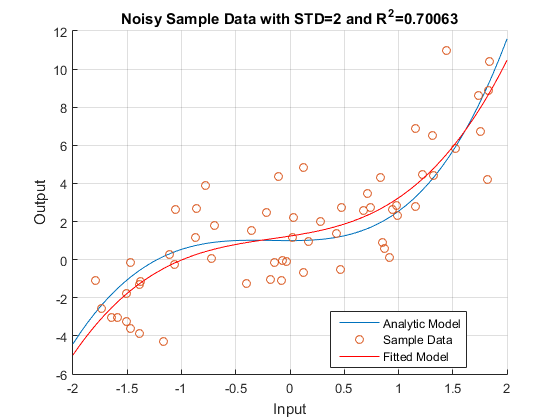
\includegraphics[width=1\linewidth]{case_best.png}
	\end{subfigure}
	\begin{subfigure}{0.49\textwidth} \centering
		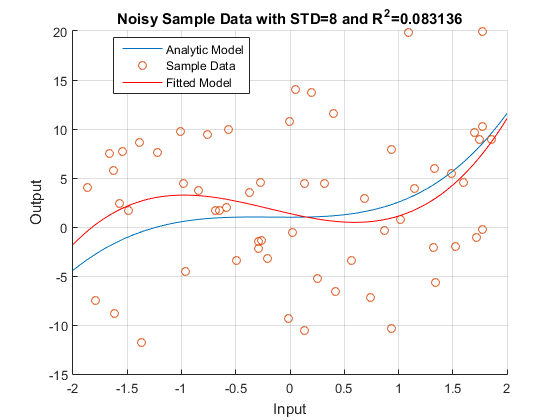
\includegraphics[width=1\linewidth]{case_worst.png}
	\end{subfigure}
	\caption{Noise Study}
	\label{probe 1}
	\end{figure}

We see that if the standard deviation of the noise is half that of the range of the input, we can get some meaningful results. If the standard deviation of the noise is double that of the range of the input, the scatter becomes random. After performing this quick study, I realized that I can plot the data from the first entry in a similar fashion and should give an indication of the noise levels in the system. I also expected to plot a best fit line similar to the plot on the left with low noise based on what we currently know.

\clearpage
%\section*{Application}

%The results from the first entry are shown in the subsequent figures. The first batch of test points that were plagued with data switching issues and the direct Q measurements performed at the end of the first entry were excluded. The dynamic pressures for probe 10 and 11, the center two probes, are plotted on top with respect to the tunnel wall pressure. The pressure readings from all the probes are plotted to show the scatter in the data in the bottom left and the probe-averaged readings are plotted in the bottom right. Note that two clusters of points are immediately visible. The points seem more randomly scatter than having a linear trend. The one-to-one relationship is plotted as a red line if visible and the x- and y-axes are equal in scale per plot. The plot below shows the results for the lowest Q setting.

%\begin{figure}[htbp] \centering
%	\begin{subfigure}{0.49\textwidth} \centering
%		\includegraphics[width=1\linewidth]{low_q_10.eps}
%	\end{subfigure}
%	\begin{subfigure}{0.49\textwidth} \centering
%		\includegraphics[width=1\linewidth]{low_q_11.eps}
%	\end{subfigure}
%	\begin{subfigure}{0.49\textwidth} \centering
%		\includegraphics[width=1\linewidth]{low_q_all.eps}
%	\end{subfigure}
%	\begin{subfigure}{0.49\textwidth} \centering
%		\includegraphics[width=1\linewidth]{low_q_avg.eps}
%	\end{subfigure}
%	\caption{Low Q Data}
%	\label{probe 1}
%	\end{figure}

%\clearpage
%The same analysis was performed for the medium Q setting and again, clusters of points seem to arise. If the bottom cluster is excluded, a linear trend could be established but looking at the full data set, the only trend seems to be a vertical line. The plot for all the probes do seem to show streaks of colors with linear trends, like the blue, green, and maroon cases, however, it is important to note that multiple cases used the same color since MATLAB rotates through only 6 colors.

%\begin{figure}[htbp] \centering
%	\begin{subfigure}{0.49\textwidth} \centering
%		\includegraphics[width=1\linewidth]{med_q_10.eps}
%	\end{subfigure}
%	\begin{subfigure}{0.49\textwidth} \centering
%		\includegraphics[width=1\linewidth]{med_q_11.eps}
%	\end{subfigure}
%	\begin{subfigure}{0.49\textwidth} \centering
%		\includegraphics[width=1\linewidth]{med_q_all.eps}
%	\end{subfigure}
%	\begin{subfigure}{0.49\textwidth} \centering
%		\includegraphics[width=1\linewidth]{med_q_avg.eps}
%	\end{subfigure}
%	\caption{Medium Q Data}
%	\label{probe 1}
%	\end{figure}

%\clearpage
%Again, the analysis was performed for the highest Q setting. The clustering is less pronounced but one cluster is prominent that seems to be an outlier. Without that cluster, a linear trend is visible. This could also be due to the larger spread in the tunnel dynamic pressure compared to the previous cases. The streaks of colors are most prominent in this case, again most likely due to the larger spread in the tunnel dynamic pressure.

%\begin{figure}[htbp] \centering
%	\begin{subfigure}{0.49\textwidth} \centering
%		\includegraphics[width=1\linewidth]{high_q_10.eps}
%	\end{subfigure}
%	\begin{subfigure}{0.49\textwidth} \centering
%		\includegraphics[width=1\linewidth]{high_q_11.eps}
%	\end{subfigure}
%	\begin{subfigure}{0.49\textwidth} \centering
%		\includegraphics[width=1\linewidth]{high_q_all.eps}
%	\end{subfigure}
%	\begin{subfigure}{0.49\textwidth} \centering
%		\includegraphics[width=1\linewidth]{high_q_avg.eps}
%	\end{subfigure}
%	\caption{High Q Data}
%	\label{probe 1}
%	\end{figure}

%\clearpage
%The analysis was performed on the test points where the dynamic pressure was directly measured at both the medium and high Q settings. The figure below shows the medium Q setting. Probe-to-probe differences seem to arise more clearly when compared directly in both where the points are concentrated as well as the slopes of a hypothetical linear best fit line.

%\begin{figure}[htbp] \centering
%	\begin{subfigure}{0.49\textwidth} \centering
%		\includegraphics[width=1\linewidth]{med_directq_10.eps}
%	\end{subfigure}
%	\begin{subfigure}{0.49\textwidth} \centering
%		\includegraphics[width=1\linewidth]{med_directq_11.eps}
%	\end{subfigure}
%	\begin{subfigure}{0.75\textwidth} \centering
%		\includegraphics[width=1\linewidth]{med_directq_all.eps}
%	\end{subfigure}
%	\caption{Direct Q Measurements at the Medium Q Setting}
%	\label{probe 1}
%	\end{figure}

%\clearpage
%This is the more interesting case because probe 11 seems to have a very flat response. The points are connected in this case to show the points changing in time. I would have expected the points to be closer together in time and therefore wander slowly in time but the plot seems to indicate otherwise.

%\begin{figure}[htbp] \centering
%	\begin{subfigure}{0.49\textwidth} \centering
%		\includegraphics[width=1\linewidth]{high_directq_10.eps}
%	\end{subfigure}
%	\begin{subfigure}{0.49\textwidth} \centering
%		\includegraphics[width=1\linewidth]{high_directq_11.eps}
%	\end{subfigure}
%	\begin{subfigure}{0.75\textwidth} \centering
%		\includegraphics[width=1\linewidth]{high_directq_all.eps}
%	\end{subfigure}
%	\caption{Direct Q Measurements at the High Q Setting}
%	\label{probe 1}
%	\end{figure}

%In conclusion, I believe that using better instrumentation in the upcoming test will give us more confidence in the noise of the system. The best case is that we are able to determine the source of this noise (fan fluctuation, temperature, weather, among others). Chad has suggested I try using a histogram and candlewick plot so I will provide an update when I can scrape up a MATLAB license that we are in such short supply of these days.


\clearpage
\section*{Low Q}
The results from the first entry are shown in the subsequent figures. The first batch of test points that were plagued with data switching issues and the direct Q measurements performed at the end of the first entry were excluded. The dynamic pressures for probe 10 and the pressure readings from all probes are plotted. Note that clusters of points are visible. The points seem more randomly scatter than having a linear trend, as evidenced by the negative slope of the curve fit. The plot below shows the results for the lowest Q setting. The uncertainty of the measurement is shown in the plus or minus band on the fitted model. The sorted points are those that were either sampled over a period of 10 minutes or more or were taken after a warm-up period of 5 minutes.

\begin{figure}[htbp] \centering
	\begin{subfigure}{0.43\textwidth} \centering
		\includegraphics[width=1\linewidth]{low_q_poly3_10.eps}
	\end{subfigure}
	\begin{subfigure}{0.43\textwidth} \centering
		\includegraphics[width=1\linewidth]{low_q_poly3_all.eps}
	\end{subfigure}
	\begin{subfigure}{0.43\textwidth} \centering
		\includegraphics[width=1\linewidth]{sort_low_q_poly3_10.eps}
	\end{subfigure}
	\begin{subfigure}{0.43\textwidth} \centering
		\includegraphics[width=1\linewidth]{sort_low_q_poly3_all.eps}
	\end{subfigure}
	%\begin{subfigure}{0.43\textwidth} \centering
	%	\includegraphics[width=1\linewidth]{low_directq_poly3_10.eps}
	%\end{subfigure}
	%\begin{subfigure}{0.43\textwidth} \centering
	%	\includegraphics[width=1\linewidth]{low_directq_poly3_all.eps}
	%\end{subfigure}
	\caption{Low Q Data with Cubic Fit. From top to bottom: all points and sorted points}
	\end{figure}

\clearpage
\section*{Medium Q}
The same is shown for the medium Q data.
\begin{figure}[htbp] \centering
	\begin{subfigure}{0.43\textwidth} \centering
		\includegraphics[width=1\linewidth]{med_q_poly3_10.eps}
	\end{subfigure}
	\begin{subfigure}{0.43\textwidth} \centering
		\includegraphics[width=1\linewidth]{med_q_poly3_all.eps}
	\end{subfigure}
	\begin{subfigure}{0.43\textwidth} \centering
		\includegraphics[width=1\linewidth]{sort_med_q_poly3_10.eps}
	\end{subfigure}
	\begin{subfigure}{0.43\textwidth} \centering
		\includegraphics[width=1\linewidth]{sort_med_q_poly3_all.eps}
	\end{subfigure}
	\begin{subfigure}{0.43\textwidth} \centering
		\includegraphics[width=1\linewidth]{med_directq_poly3_10.eps}
	\end{subfigure}
	\begin{subfigure}{0.43\textwidth} \centering
		\includegraphics[width=1\linewidth]{med_directq_poly3_all.eps}
	\end{subfigure}
	\caption{Medium Q Data with Cubic Fit. From top to bottom: all, sorted, and direct reading points}
	\end{figure}

\clearpage
\section*{High Q}

\begin{figure}[htbp] \centering
	\begin{subfigure}{0.43\textwidth} \centering
		\includegraphics[width=1\linewidth]{high_q_poly3_10.eps}
	\end{subfigure}
	\begin{subfigure}{0.43\textwidth} \centering
		\includegraphics[width=1\linewidth]{high_q_poly3_all.eps}
	\end{subfigure}
	\begin{subfigure}{0.43\textwidth} \centering
		\includegraphics[width=1\linewidth]{sort_high_q_poly3_10.eps}
	\end{subfigure}
	\begin{subfigure}{0.43\textwidth} \centering
		\includegraphics[width=1\linewidth]{sort_high_q_poly3_all.eps}
	\end{subfigure}
	\begin{subfigure}{0.43\textwidth} \centering
		\includegraphics[width=1\linewidth]{high_directq_poly3_10.eps}
	\end{subfigure}
	\begin{subfigure}{0.43\textwidth} \centering
		\includegraphics[width=1\linewidth]{high_directq_poly3_all.eps}
	\end{subfigure}
	\caption{High Q Data with Cubic Fit. From top to bottom: all, sorted, and direct reading points}
	\end{figure}

\clearpage
\section*{Histogram}
Below is a plot of histograms for both the tunnel dynamic pressures and the probe dynamic pressures where the low, medium, and high Q cases are shown in each row, respectively, and the tunnel and probe dynamic pressures are shown left to right. The bin size is equal to the measurement uncertainty. Two distributions are plotted and their relative ``goodness of fit'' is shown in the legend, where 1 is the best fit. I don't know why the metric on the histogram on the bottom right exceeded 1.

\begin{figure}[htbp] \centering
	\begin{subfigure}{0.43\textwidth} \centering
		\includegraphics[width=1\linewidth]{low_q_hist_tun.eps}
	\end{subfigure}
	\begin{subfigure}{0.43\textwidth} \centering
		\includegraphics[width=1\linewidth]{low_q_hist_probe.eps}
	\end{subfigure}
	\begin{subfigure}{0.43\textwidth} \centering
		\includegraphics[width=1\linewidth]{med_q_hist_tun.eps}
	\end{subfigure}
	\begin{subfigure}{0.43\textwidth} \centering
		\includegraphics[width=1\linewidth]{med_q_hist_probe.eps}
	\end{subfigure}
	\begin{subfigure}{0.43\textwidth} \centering
		\includegraphics[width=1\linewidth]{high_q_hist_tun.eps}
	\end{subfigure}
	\begin{subfigure}{0.43\textwidth} \centering
		\includegraphics[width=1\linewidth]{high_q_hist_probe.eps}
	\end{subfigure}
	\caption{Histogram of Pressure Data}
	\end{figure}

\clearpage
\section*{Summary of Results}

Tabulated below are the results from the curve-fitting on probe 10. Fit order refers to whether the fit is linear (1st order) or cubic (3rd order). R$^2$ is a metric of the "goodness" of fit. RMSE stands for the root mean square of the error and is a measure of the standard deviation of the error, or the noise of the system. NU ratio is something I made up which stands for the noise-to-uncertainty ratio and is a measure of the system noise to the instrument uncertainty.

\begin{center} \begin{tabular}{|c|c|c|c|c|} \hline 
Dynamic Pressure & Fit Order & R$^2$ & RMSE [psf] & NU Ratio \tabularnewline \hline \hline 
Low    & 1 & 0.063 & 0.047 & 0.76 \tabularnewline \hline 
Low    & 3 & 0.065 & 0.048 & 0.77 \tabularnewline \hline 
Medium & 1 & 0.090 & 0.213 & 3.44 \tabularnewline \hline 
Medium & 3 & 0.193 & 0.204 & 3.29 \tabularnewline \hline 
High   & 1 & 0.198 & 0.397 & 6.40 \tabularnewline \hline 
High   & 3 & 0.270 & 0.384 & 6.19 \tabularnewline \hline
\end{tabular} \par\end{center}

From these results, the low dynamic pressure case exhibits the most random behavior, especially from the negative linear trends. The medium but especially the high dynamic pressure case seems to indicate that the system noise is quite high, higher than the instrument uncertainty. Cubic fits produce better fits at the medium and high dynamic pressures suggesting the data is more nonlinear than linear.

\clearpage
\section*{Turbulence Intensity}

Given a velocity difference, the associated difference in dynamic pressure can be calculated using the derivation shown below. If two measurements are taken, their dynamic pressures can be described as a function of their respective velocities.

$$ q_1 = \frac{1}{2}\rho v_1^2 $$
$$ q_2 = \frac{1}{2}\rho v_2^2 $$

If density is assumed constant, the two measurements can be related as follows:

$$ q_2 - q_1 = \frac{1}{2}\rho v_2^2 - \frac{1}{2}\rho v_1^2 $$
\begin{equation} \Delta q = \frac{1}{2}\rho (v_2^2 - v_1^2) \label{delq} \end{equation}

If the difference between the two velocity measurements are small, they too can be related with a turbulence intensity measurement $T_i$, where turbulence intensity is defined as the ratio between the standard deviation of the velocity, $\Delta v$, and the mean velocity, $v$ ($T_i = \Delta v / v$). 
$$ v_2 - v_1 = \Delta v = v_i\cdot T_i $$
$$ v_2 = T_i\cdot v_1 + v_1 $$
\begin{equation} v_2 = (T_i + 1)\cdot v_1 \label{vdef} \end{equation}

\Cref{delq,vdef} can be combined and the subscripts dropped
\begin{align*}
\Delta q &= \frac{1}{2}\rho (v_2^2 - v_1^2) \\
&=  \frac{1}{2}\rho (v_1^2(T_i + 1)^2  - v_1^2) \\
&=  \frac{1}{2}\rho ( v^2(T_i^2 + 2 T_i + 1 - 1)) \\
\Delta q &=  \frac{1}{2}\rho v^2(T_i^2 + 2 T_i) \numberthis \label{fin}
\end{align*}

\Cref{fin} describes the change in pressure given a turbulence intensity, $T_i$, a mean velocity, $v$, and a density, $\rho$. Given Tina's measured turbulence intensity without the net installed of 1.5\%, the turbulence quantities are compared with the measured quantities at the given velocities. The subscript $t$ denotes turbulence quantities, the subscript $i$ denotes the calculated ideal value (given incompressible flow), and the subscript $m$ denotes the measured values from this experiment. The ideal dynamic pressure, $q_i$, is compared with the measured average dynamic pressure, $\bar{q}_m$, by a percent difference from the ideal. The standard deviation of the dynamic pressure due to turbulence, $\Delta q_t$, is compared with the measured standard deviation of the experiment (from cubic fit of probe 10), $\Delta q_m$, by a ratio $\Delta q_t / \Delta q_m$. The values are tabulated below.

\begin{center} \begin{tabular}{|c|c|c|c|c|c|c|c|} \hline 
$v$ [ft/s] & $\Delta v_t$ [ft/s] & $q_i$ [psf] & $\bar{q}_m [psf]$ & Difference $q$ & $\Delta q_t$ [psf] & $\Delta q_m$ [psf]& Ratio $\Delta q$ \tabularnewline \hline \hline 
140        & 2.10                & 23.30     & 21.76             & -6.64\%        & 0.704              & 0.048             & 0.07 \tabularnewline \hline 
95         & 1.43                & 10.73     & 10.20             & -4.93\%        & 0.324              & 0.204             & 0.63 \tabularnewline \hline 
50         & 0.75                &  2.97     &  2.96             & -0.35\%        & 0.090              & 0.384             & 4.27 \tabularnewline \hline 
\end{tabular} \par\end{center}

The first thing to note is that the incompressible values for dynamic pressure match experiment well at the lowest $q$ but get high at the middle and highest values of $q$. Maybe there are compressible effects at the wall. The second observation is that the "noise" of our system at the lowest $q$ was 4 times greater than that of the turbulence Tina measured but at middle to high $q$, the "noise" of our system is much smaller than the turbulence Tina measured. To add weight to this analysis, we should consider the uncertainty of the hot-wire measurement.

\end{document}
